\documentclass[12pt,a4paper]{article}
\usepackage[margin=2.5cm]{geometry}
\usepackage{lmodern}
\usepackage[T1]{fontenc}
\usepackage{amsmath,amssymb}
\usepackage{booktabs,array,tabularx}
\usepackage{enumitem}
\usepackage{xcolor}
\usepackage{graphicx}
\usepackage[most]{tcolorbox}
\usepackage{titlesec}
\usepackage[colorlinks=true,linkcolor=black,urlcolor=blue!50!black]{hyperref}

\definecolor{headblue}{RGB}{38,70,120}
\titleformat{\section}{\Large\bfseries\color{headblue}}{\thesection}{0.8em}{}[{\color{black}\titlerule}]
\titleformat{\subsection}{\large\bfseries}{\thesubsection}{0.8em}{}
\setlength{\parindent}{0pt}
\setlength{\parskip}{6pt}

\newcommand{\mdesc}[1]{\par{\textit{Meaning:} #1}\par}
\newtcolorbox{objbox}{colback=blue!3,colframe=headblue!60,boxrule=0.5pt,arc=2mm,left=2mm,right=2mm,top=1mm,bottom=1mm}
\newtcolorbox{whatsnew}{colback=orange!4,colframe=orange!60!black,boxrule=0.5pt,arc=2mm,left=2mm,right=2mm,top=1mm,bottom=1mm}

\begin{document}

\begin{center}
{\LARGE\bfseries\color{headblue} EV Charging Network Optimisation}\\[6pt]
{\large Formulation 4: EV $\rightarrow$ charger (FCS / MCS) assignment + mobile charger routing\\ with a use segment (personal / commercial) and a continuous income attribute}\\[4pt]
{\normalsize CP 320 Operations Research for Mobility Management, course project}\\[2pt]
{\normalsize 22 November 2026}
\end{center}
\vspace{4pt}

\begin{whatsnew}
\textbf{What is new.} Formulation 4 is formulation 3 (\texttt{main\_formulation\_3.pdf}) plus one more customer attribute, the \textbf{use segment} $s_i\in\{\mathrm P,\mathrm C\}$ of every EV: \emph{personal} (private car) or \emph{commercial} (taxi, ride-hailing, fleet car). It follows the extension proposed in Section~4.14 (calibration and extensions) of the formulation-3 comprehensive report: a taxi's value of time is the vehicle's lost earnings, not household income. The segment changes how each customer values money, time and queueing; the variables and constraints (1)--(23) are those of formulation 3. Section~\ref{sec:calib} recommends the distributions of the two attributes from Indian data, Section~\ref{sec:exp} lists the experiments.
\end{whatsnew}

%=====================================================================
\section{Problem Statement}

Given a small road network, the network operator wants to assign each EV with its respective demand either to a fixed charging station or a mobile charging station.

\hspace{1.5em}During the time interval $[0,T]$ a set of parked EVs raise charging requests. Each request must be served by exactly one resource: either the EV drives itself to a fixed charging station (FCS, 2 guns of 22\,kW each), or a mobile charging van (MCS) leaves the depot, drives to the EV, charges it (one EV at a time) and moves on, returning to the depot by $T$.

Every EV $i$ carries two attributes, both known in advance:
\begin{itemize}[itemsep=1pt]
  \item a \textbf{use segment} $s_i\in\{\mathrm P,\mathrm C\}$: P = personal car, C = commercial car (taxi, ride-hailing, fleet);
  \item an \textbf{income index} $\theta_i\in[0,1]$: the household's position in the income distribution, 0 = lowest, 1 = highest.
\end{itemize}
The two attributes change how a customer feels a rupee and a minute:
\begin{itemize}[itemsep=1pt]
  \item within a segment, a lower-income customer feels every rupee more and values time less, as in formulation 3;
  \item a \emph{personal} driver's minute depends on where the driver is: driving, queueing and charging at a station take the driver's time, while a van charges the parked car with the driver free;
  \item a \emph{commercial} car earns nothing while it is out of service: every minute of driving to a station, queueing, charging, or waiting for and being charged by a van costs the same lost earnings (the \emph{downtime} rate). A van gives a taxi no ``driver-free'' benefit; it only saves downtime.
\end{itemize}
Who ends up at an FCS and who gets a van follows from these sensitivities, the operator's costs and the limited guns and vans.

We decide -
\begin{enumerate}[itemsep=2pt]
  \item Who serves each EV.
  \item The order in which each van visits its EVs.
  \item The time every charging session starts.
\end{enumerate}

\begin{objbox}
{\color{headblue}\textbf{Our Objective}}\\
Minimise the operator's cost plus the cost that customers perceive, where each customer weighs money and time according to their segment and income.
\end{objbox}

%=====================================================================
\section{Assumptions}
\begin{enumerate}[itemsep=2pt]
  \item All requests of the planning period are known at time 0; request $i$ becomes active at $r_i$ (request release time). All times are non-negative real numbers, measured in minutes, in $[0,T]$.
  \item An EV served by an FCS drives there itself (one way) on its own battery, waits for a free gun, and stays until charged. An EV can only use an FCS within its remaining range.
  \item Customer $i$ waits at most $W_i$ minutes at a station for a free gun; $W_i$ depends on segment and income.
  \item An EV served by an MCS stays parked at its location; the van comes to it.
  \item Each FCS gun and each MCS charges one EV at a time, with no pre-emption.
  \item A van's driving energy and delivered energy come from the same battery; there is no recharging of the van during the peak.
  \item Every request must be fully charged by $T$ (hard).
  \item Charging power is constant.
  \item \textbf{(changed)} Every customer has a use segment $s_i\in\{\mathrm P,\mathrm C\}$ and an income index $\theta_i\in[0,1]$, both known in advance. The pairs $(s_i,\theta_i)$ are drawn independently: $s_i$ is commercial with probability $\pi_{\mathrm C}$, and $\theta_i$ given $s_i$ follows a distribution $F_{s_i}$ on $[0,1]$.
  \item \textbf{(changed)} The attributes act only through three sensitivities, known functions of $(\theta,s)$: the money sensitivity $\mu^{s}(\theta)$ is non-increasing in $\theta$, the value of time $c^{a,s}(\theta)$ of each activity $a$ is non-decreasing and the queue tolerance $W^{s}(\theta)$ is non-increasing.
  \item \textbf{(new)} A commercial car's time is valued at its downtime rate $\omega(\theta)=c^{\mathrm D,\mathrm C}(\theta)=c^{\mathrm C,\mathrm C}(\theta)=c^{\mathrm V,\mathrm C}(\theta)$ whatever the activity; queueing costs at least as much, $c^{\mathrm Q,\mathrm C}(\theta)\ge\omega(\theta)$.
  \item \textbf{(new)} The segment changes no network data: positions, energy demand $E_i$, request time $r_i$ and range $R_i$ come from the EV-Solomon files for both segments, and both segments pay the same tariffs. So any difference between segments in the results comes from the sensitivities and the income distributions only.
  \item Customers pay a tariff per kWh: $p^{\mathrm F}$ at an FCS and $p^{\mathrm M}\ge p^{\mathrm F}$ for the van service (a premium for charging at the door). An FCS user also pays for driving to the station.
  \item The operator minimises its own cost plus the customers' perceived cost. Tariff revenue is not counted as a gain for the operator.
\end{enumerate}

%=====================================================================
\newpage
\section{Sets, parameters and decision variables}

\subsection*{Sets}
\begin{tabularx}{\textwidth}{@{}>{\raggedright\arraybackslash}p{4.6cm}X@{}}
\toprule
\textbf{Notation} & \textbf{Description} \\
\midrule
$I=\{1,\dots,n\}$ & Set of EV charging requests. \\[2pt]
$\mathcal S=\{\mathrm P,\mathrm C\}$ & \textbf{(new)} Use segments: personal, commercial. $I^{\mathrm P}=\{i: s_i=\mathrm P\}$, $I^{\mathrm C}=\{i: s_i=\mathrm C\}$, $I=I^{\mathrm P}\cup I^{\mathrm C}$. \\[2pt]
$F$,\ \ $|F|=12$ (or $24$) & Set of fixed charging stations (FCS). Dataset: 12 stations in the 100-EV files, 24 in the 200-EV files. \\[2pt]
$G_f$,\ \ $|G_f|=2$ & Set of guns at FCS $f$. $G=\bigcup_{f\in F}G_f$; $f(g)$ is the station of gun $g$. \\[2pt]
$F_i=\{f\in F: d_{if}\le R_i\}$ & Set of FCS that EV $i$ can reach given its remaining range. \\[2pt]
$G_i=\bigcup_{f\in F_i}G_f$ & Set of guns that EV $i$ can use. \\[2pt]
$M$,\ \ $|M|=5$ (or $12$) & Set of mobile charging vans. \\[2pt]
$0,\ n+1$ & Start and end depot nodes (the same place). \\[2pt]
$N=\{0\}\cup I\cup\{n+1\}$ & Set of routing nodes. \\[2pt]
$A$ & Allowed van arcs: $A=\{(i,j): i\in\{0\}\cup I,\ j\in I\cup\{n+1\},\ i\ne j,\ (i,j)\ne(0,n+1)\}$. \\[2pt]
$P_g=\{(i,j)\in I^2: i<j,\ g\in G_i\cap G_j\}$ & EV pairs that could share gun $g$ (and must then be sequenced). \\[2pt]
$G^{+}=\{g\in G: g\in G_i \text{ for some } i\}$ & Guns that at least one EV can reach. \\[2pt]
$\mathcal A=\{\mathrm D,\mathrm Q,\mathrm C,\mathrm V\}$ & Activities that take a customer's time: driving to an FCS, queueing at an FCS, charging at an FCS, and the car parked while it waits for and is charged by a van. \\
\bottomrule
\end{tabularx}

\subsection*{Parameters (unchanged from formulation 3)}
{\small
\begin{tabularx}{\textwidth}{@{}>{\raggedright\arraybackslash}p{4.6cm}X@{}}
\toprule
\textbf{Notation} & \textbf{Description} \\
\midrule
$E_i$ & Energy demand of EV $i$ (kWh). Dataset: Solomon DEMAND mapped linearly to $[10,40]$. \\[2pt]
$r_i$ & Request (release) time (minutes). Dataset: Solomon READY TIME. \\[2pt]
$R_i$ & Remaining driving range of EV $i$ (km); 15\,\% of the EVs cannot reach any FCS (``stranded'', $F_i=\emptyset$). \\[2pt]
$P^{\mathrm F},\ P^{\mathrm M}$ & Charging power of an FCS gun and of an MCS (kW). \\[2pt]
$\tau^{\mathrm F}_i=\dfrac{60E_i}{P^{\mathrm F}},\ \tau^{\mathrm M}_i=\dfrac{60E_i}{P^{\mathrm M}}$ & Charging duration of EV $i$ at an FCS and by an MCS (minutes); $\tau^{\mathrm M}_i<\tau^{\mathrm F}_i$ since $P^{\mathrm M}>P^{\mathrm F}$. \\[2pt]
$d_{if},\ t_{if}$ & Road distance (km) and travel time (min) from EV $i$ to FCS $f$. \\[2pt]
$d_{ij},\ t_{ij}$ & Road distance (km) and travel time (min) between routing nodes. \\[2pt]
$v$ & Travel speed (km/h). \\[2pt]
$B_m,\ Q_m$ & Usable battery (kWh) and maximum number of EVs (seats) of van $m$. \\[2pt]
$\beta,\ \eta$ & Van driving consumption (kWh/km) and charging efficiency. \\[2pt]
$T$ & Length of the planning period (min); Solomon's depot due date, unchanged. \\[2pt]
$c^{\mathrm{EV}},\ c^{\mathrm M}$ & Cost per km of EV driving (paid by the customer) and of van driving (Rs/km). \\[2pt]
$c^{\mathrm F}_m$ & Fixed dispatch cost of van $m$ (Rs). \\[2pt]
$\pi^{\mathrm F},\ \pi^{\mathrm M}$ & Operator's cost per kWh of grid energy at an FCS and of van battery energy (Rs/kWh). \\[2pt]
$p^{\mathrm F}\le p^{\mathrm M}$ & Tariffs per kWh at an FCS and for the van service (Rs/kWh), the same for both segments. \\[2pt]
$M^{\mathrm M}_{ij}=T+\tau^{\mathrm M}_i+t_{ij},\ M^{\mathrm F}_i=T+\tau^{\mathrm F}_i$ & Big-$M$ constants (minutes). \\
\bottomrule
\end{tabularx}}

\newpage
\subsection*{Customer attributes and sensitivities (new and changed in formulation 4)}
{\small
\begin{tabularx}{\textwidth}{@{}>{\raggedright\arraybackslash}p{4.6cm}X@{}}
\toprule
\textbf{Notation} & \textbf{Description} \\
\midrule
$s_i\in\{\mathrm P,\mathrm C\}$ & \textbf{(new)} Use segment of EV $i$. Data: $s_i=\mathrm C$ with probability $\pi_{\mathrm C}$ (the share of commercial cars among \emph{public charging requests}, Section~\ref{sec:calib}). \\[2pt]
$\theta_i\in[0,1]$ & Income index of EV $i$'s household. Data: $\theta_i\mid s_i\sim F_{s_i}$, a Beta$(a_{s},b_{s})$ distribution per segment (Section~\ref{sec:calib}). The same EV number has the same $(s_i,\theta_i)$ in every file of a Solomon class. \\[2pt]
$\mu_i=\mu^{s_i}(\theta_i)>0$ & Money sensitivity (Rs perceived per Rs paid). $\mu^{s}(\cdot)$ non-increasing. \\[2pt]
$c^{a}_i=c^{a,s_i}(\theta_i)\ge0$,\ \ $a\in\mathcal A$ & Value of time of customer $i$ in activity $a$ (Rs/min). Each $c^{a,s}(\cdot)$ is non-decreasing.
\newline\textbf{Personal} ($s=\mathrm P$), as formulation 3: $c^{\mathrm Q,\mathrm P}>c^{\mathrm D,\mathrm P}$ (queueing is worse than driving) and $c^{\mathrm V,\mathrm P}\le c^{\mathrm C,\mathrm P}$ (a minute with the driver free costs less than a minute at the station), the gap not shrinking with income, $c^{\mathrm V,\mathrm P\prime}\le c^{\mathrm C,\mathrm P\prime}$.
\newline\textbf{Commercial} ($s=\mathrm C$): one downtime rate $\omega(\theta)=c^{\mathrm D,\mathrm C}(\theta)=c^{\mathrm C,\mathrm C}(\theta)=c^{\mathrm V,\mathrm C}(\theta)$ and $c^{\mathrm Q,\mathrm C}(\theta)=\omega(\theta)+\delta(\theta)$ with $\delta(\theta)\ge0$ (a queue keeps the driver with the car and its end is uncertain). \\[2pt]
$W_i=W^{s_i}(\theta_i)\ge0$ & Longest queue customer $i$ accepts at an FCS (minutes). $W^{s}(\cdot)$ non-increasing. \\
\bottomrule
\end{tabularx}}

\textbf{Shape of the sensitivity functions.} The model needs only the directions above. In the code each function is a straight line in $\theta$ between its value at $\theta=0$ and at $\theta=1$, \emph{with its own end points per segment}:
\begin{gather*}
\mu^{s}(\theta)=\mu^{s,0}+(\mu^{s,1}-\mu^{s,0})\,\theta,\qquad
W^{s}(\theta)=W^{s,0}+(W^{s,1}-W^{s,0})\,\theta,\\
c^{a,s}(\theta)=c^{a,s,0}+(c^{a,s,1}-c^{a,s,0})\,\theta,\qquad s\in\mathcal S,\ a\in\mathcal A .
\end{gather*}
Because $(s_i,\theta_i)$ are data, $\mu_i$, $c^{a}_i$ and $W_i$ are numbers before the model is solved: the model stays a linear MILP of exactly the size of formulation 3. The end points are kept symbolic here; the values used in the experiments are in \texttt{common/f4\_params.json}.

\subsection*{Decision variables (unchanged)}
\begin{tabularx}{\textwidth}{@{}>{\raggedright\arraybackslash}p{4.6cm}X@{}}
\toprule
\textbf{Notation} & \textbf{Description} \\
\midrule
$y_{ig}\in\{0,1\}$ & 1 if EV $i$ is charged at gun $g\in G_i$. \\[2pt]
$z_{im}\in\{0,1\}$ & 1 if EV $i$ is served by van $m$. \\[2pt]
$x_{ijm}\in\{0,1\}$ & 1 if van $m$ traverses arc $(i,j)\in A$. \\[2pt]
$u_m\in\{0,1\}$ & 1 if van $m$ is dispatched. \\[2pt]
$o_{ij}\in\{0,1\}$ & For EV pairs $i<j$ sharing a gun, 1 if $i$ is charged before $j$. \\[2pt]
$S_i\ge0$ & Start time of EV $i$'s charging session (minute). \\[2pt]
$q^{\mathrm F}_i\ge0$,\ \ $q^{\mathrm M}_i\ge0$ & Queue at the FCS / wait for the van before charging starts (minutes). \\
\bottomrule
\end{tabularx}

Short-hands: $Y_{if}=\sum_{g\in G_f}y_{ig}$, $y_i=\sum_{g\in G_i}y_{ig}$, $z_i=\sum_{m\in M}z_{im}$, $C_i=S_i+\tau^{\mathrm F}_i y_i+\tau^{\mathrm M}_i z_i$. The time from request to full charge, $C_i-r_i=\sum_{f}t_{if}Y_{if}+q^{\mathrm F}_i+q^{\mathrm M}_i+\tau^{\mathrm F}_iy_i+\tau^{\mathrm M}_iz_i$, is for a commercial car its \textbf{downtime}. The money customer $i$ pays is $\text{Pay}_i=c^{\mathrm{EV}}\sum_{f}d_{if}Y_{if}+p^{\mathrm F}E_iy_i+p^{\mathrm M}E_iz_i$.

%=====================================================================
\section{Objective}

\begin{equation}
\begin{aligned}
\min\ Z \;=\;& \underbrace{\sum_{i\in I}\mu_i\,c^{\mathrm{EV}}\sum_{f\in F_i}d_{if}Y_{if}}_{Z_1:\ \text{EV driving (perceived)}}
+\underbrace{c^{\mathrm M}\sum_{m\in M}\sum_{(i,j)\in A}d_{ij}x_{ijm}}_{Z_2:\ \text{van driving}}
+\underbrace{\sum_{m\in M}c^{\mathrm F}_mu_m}_{Z_3:\ \text{van dispatch}}\\
&+\underbrace{\pi^{\mathrm F}\sum_{i\in I}E_i\,y_i+\pi^{\mathrm M}\sum_{i\in I}\frac{E_i}{\eta}\,z_i}_{Z_4:\ \text{operator energy}}
+\underbrace{\sum_{i\in I}\mu_i\,E_i\big(p^{\mathrm F}y_i+p^{\mathrm M}z_i\big)}_{Z_5:\ \text{tariff (perceived)}}\\
&+\underbrace{\sum_{i\in I}\Big(c^{\mathrm D}_i\sum_{f\in F_i}t_{if}Y_{if}+c^{\mathrm Q}_i\,q^{\mathrm F}_i+c^{\mathrm C}_i\,\tau^{\mathrm F}_iy_i+c^{\mathrm V}_i\big(q^{\mathrm M}_i+\tau^{\mathrm M}_iz_i\big)\Big)}_{Z_6:\ \text{time (perceived)}}
\end{aligned}\label{eq:obj}
\end{equation}
with $\mu_i=\mu^{s_i}(\theta_i)$, $c^{a}_i=c^{a,s_i}(\theta_i)$. $Z_2+Z_3+Z_4$ is the \textbf{operator's cost}; $Z_1+Z_5+Z_6$ is the \textbf{customers' perceived cost}. The form is that of formulation 3; what changes is that every customer coefficient now depends on the segment as well as on income.

For a commercial EV the time term $Z_6$ collapses to one downtime price:
\[
Z_{6,i}\big|_{s_i=\mathrm C}=\omega(\theta_i)\,(C_i-r_i)+\delta(\theta_i)\,q^{\mathrm F}_i ,
\]
lost earnings for every minute out of service, plus the extra cost of a queue. For a personal EV it keeps the four activity rates of formulation 3; in particular the van's charging minutes are priced at the driver-free rate $c^{\mathrm V}_i\le c^{\mathrm C}_i$.

%---------------------------------------------------------------------
\subsection{How segment and income enter the decision}
\label{sec:theory}

Fix the rest of the plan and compare serving EV $i$ at FCS $f$ with queue $q^{\mathrm F}_i$, or by a van with wait $q^{\mathrm M}_i$. Write $\Pi_i=(p^{\mathrm M}-p^{\mathrm F})E_i-c^{\mathrm{EV}}d_{if}$ for the extra money the van costs the customer and $\kappa_i=(\pi^{\mathrm M}/\eta-\pi^{\mathrm F})E_i+c^{\mathrm M}\times$(extra van km) ($+c^{\mathrm F}_m$ if the van would not leave otherwise) for the operator's extra cost; neither depends on the customer. The van is the better choice when $\Delta_i<0$.

\textbf{Personal EV} (as formulation 3):
\[
\Delta^{\mathrm P}_i(\theta)=\mu^{\mathrm P}(\theta)\,\Pi_i+\kappa_i-\Big[c^{\mathrm D,\mathrm P}(\theta)\,t_{if}+c^{\mathrm Q,\mathrm P}(\theta)\,q^{\mathrm F}_i+c^{\mathrm C,\mathrm P}(\theta)\,\tau^{\mathrm F}_i-c^{\mathrm V,\mathrm P}(\theta)\big(q^{\mathrm M}_i+\tau^{\mathrm M}_i\big)\Big].
\]

\textbf{Commercial EV.} With $\omega=c^{\mathrm D}=c^{\mathrm C}=c^{\mathrm V}$ and $c^{\mathrm Q}=\omega+\delta$,
\[
\Delta^{\mathrm C}_i(\theta)=\mu^{\mathrm C}(\theta)\,\Pi_i+\kappa_i-\omega(\theta)\,D_i-\delta(\theta)\,q^{\mathrm F}_i,\qquad
D_i=\underbrace{t_{if}+q^{\mathrm F}_i+\tau^{\mathrm F}_i}_{\text{downtime at the FCS}}-\underbrace{\big(q^{\mathrm M}_i+\tau^{\mathrm M}_i\big)}_{\text{downtime with the van}} .
\]
$D_i$ is the downtime the van saves. Off-peak ($q^{\mathrm F}_i=0$) it is $D_i=t_{if}+60E_i\big(\tfrac1{P^{\mathrm F}}-\tfrac1{P^{\mathrm M}}\big)-q^{\mathrm M}_i$: the drive plus the faster charging, minus the wait for the van.

\textbf{Consequences.}
\begin{enumerate}[itemsep=2pt]
  \item \emph{A taxi takes a van only to save downtime.} If the van wait exceeds the drive plus the power gain ($D_i\le0$ off-peak), a commercial EV never prefers the van, whatever its income: $\Delta^{\mathrm C}_i\ge\mu^{\mathrm C}\Pi_i+\kappa_i>0$ when $\Pi_i>0$.
  \item \emph{Queues, not income, push commercial EVs to vans.} $\partial\Delta^{\mathrm C}_i/\partial q^{\mathrm F}_i=-(\omega+\delta)<0$: every minute of station queue raises the van's value to a taxi at the full downtime rate. In the peak the van becomes attractive to commercial EVs that would never take it off-peak.
  \item \emph{The driver-free benefit belongs to personal cars.} Compare a personal and a commercial EV in the same situation with the same time values at the station ($c^{\mathrm D,\mathrm P}=c^{\mathrm C,\mathrm P}=\omega$ and $c^{\mathrm Q,\mathrm P}=\omega+\delta$): then, since $c^{\mathrm V,\mathrm P}\le c^{\mathrm C,\mathrm P}=\omega$,
  \[
  \Delta^{\mathrm C}_i-\Delta^{\mathrm P}_i=\big(\mu^{\mathrm C}-\mu^{\mathrm P}\big)\Pi_i+\big(\omega-c^{\mathrm V,\mathrm P}\big)\big(q^{\mathrm M}_i+\tau^{\mathrm M}_i\big)\ \ge\ \big(\mu^{\mathrm C}-\mu^{\mathrm P}\big)\Pi_i .
  \]
  With equal money sensitivity the commercial EV values the van less, by exactly the driver-free discount on the van's minutes. Commercial EVs win van seats only through a larger downtime rate or longer queues.
  \item \emph{Income threshold per segment.} With straight-line sensitivities both $\Delta^{\mathrm P}_i$ and $\Delta^{\mathrm C}_i$ are linear in $\theta$, so for a given schedule each segment has one income threshold. For the commercial segment
  \[
  \theta^{*}_{i,\mathrm C}=\frac{\mu^{\mathrm C,0}\,\Pi_i+\kappa_i-\omega^{0}D_i-\delta^{0}q^{\mathrm F}_i}{(\mu^{\mathrm C,0}-\mu^{\mathrm C,1})\,\Pi_i+(\omega^{1}-\omega^{0})\,D_i+(\delta^{1}-\delta^{0})\,q^{\mathrm F}_i}
  \]
  (denominator positive when $\Pi_i>0$, $D_i>0$ and $\delta$ non-decreasing): above it the van is chosen. It falls with the queue $q^{\mathrm F}_i$ and with the saved downtime $D_i$, and rises with the van premium $\Pi_i$ and the operator's extra cost $\kappa_i$. The personal threshold $\theta^{*}_{i,\mathrm P}$ is that of formulation 3 (Section~4.1 there).
  \item \emph{Who gets the scarce vans.} Vans are limited ($\sum_mQ_m$, battery, time). The model gives the van slots to the EVs with the most negative $\Delta_i$: off-peak these are high-income personal EVs (driver-free benefit growing with income); in the peak, commercial EVs facing long queues compete for the same seats. Low-income customers of both segments absorb the station queues; where $W^{\mathrm C}(\theta)\le W^{\mathrm P}(\theta)$, a commercial EV is the first to be moved when a queue grows.
  \item \emph{The segment mix matters.} With more commercial EVs ($\pi_{\mathrm C}$ larger) fewer customers value the driver-free benefit, so off-peak van demand falls; in the peak more customers value downtime, so peak van demand rises. The calibrated $\pi_{\mathrm C}$ (Section~\ref{sec:calib}) is high, so the segment mix is a first-order input of the results.
\end{enumerate}
If both segments had the same sensitivity functions, $s_i$ would not matter and the model would be formulation 3 with income distribution $(1-\pi_{\mathrm C})F_{\mathrm P}+\pi_{\mathrm C}F_{\mathrm C}$.

%=====================================================================
\section{Constraints (as formulation 3)}

\subsection{Assignment}
\begin{equation}
y_i+z_i=\sum_{g\in G_i}y_{ig}+\sum_{m\in M}z_{im}=1\qquad\forall i\in I \label{eq:assign}
\end{equation}
\mdesc{Every request is served by exactly one resource; an EV that reaches no FCS ($G_i=\emptyset$) is forced onto a van, whatever its segment or income.}

\subsection{Fixed charging stations (continuous time)}
\begin{equation}
S_i\ \ge\ r_i+\sum_{f\in F_i}t_{if}\,Y_{if}\qquad\forall i\in I \label{eq:fcsarr}
\end{equation}
\begin{align}
q^{\mathrm F}_i+q^{\mathrm M}_i &= S_i-r_i-\sum_{f\in F_i}t_{if}\,Y_{if} && \forall i\in I \label{eq:wait}\\
q^{\mathrm F}_i &\le W_i\,y_i && \forall i\in I \label{eq:waitF}\\
q^{\mathrm M}_i &\le T\,z_i && \forall i\in I \label{eq:waitM}
\end{align}
\mdesc{\eqref{eq:fcsarr}: an FCS user starts after its request and its drive. \eqref{eq:wait}: the time between arrival (or request) and start is the waiting time. \eqref{eq:waitF}: an FCS user queues at most $W_i=W^{s_i}(\theta_i)$, its own segment- and income-dependent limit. \eqref{eq:waitM}: only an MCS user waits for a van.}

\begin{align}
S_j &\ge S_i+\tau^{\mathrm F}_i-M^{\mathrm F}_i\,(3-y_{ig}-y_{jg}-o_{ij}) && \forall g\in G,\ (i,j)\in P_g \label{eq:disj1}\\
S_i &\ge S_j+\tau^{\mathrm F}_j-M^{\mathrm F}_j\,(2-y_{ig}-y_{jg}+o_{ij}) && \forall g\in G,\ (i,j)\in P_g \label{eq:disj2}
\end{align}
\mdesc{No two EVs overlap on the same gun (disjunctive sequencing).}

\begin{equation}
\sum_{i\in I}\tau^{\mathrm F}_i\,y_{ig}\ \le\ T-\min_{i:\,g\in G_i}\Big(r_i+t_{if(g)}\Big)\qquad\forall g\in G^{+} \label{eq:gunload}
\end{equation}
\mdesc{Valid inequality: the charging time on one gun fits in the time it is available.}

\begin{equation}
\sum_{i\in I}y_{ig_1}\ \ge\ \sum_{i\in I}y_{ig_2}\qquad\forall f\in F,\ G_f=\{g_1,g_2\} \label{eq:gunsym}
\end{equation}
\mdesc{Symmetry breaking between the identical guns of a station.}

\subsection{MCS routing}
\begin{align}
\sum_{j:(0,j)\in A}x_{0jm} &= u_m && \forall m\in M \label{eq:out}\\
\sum_{i:(i,n+1)\in A}x_{i,n+1,m} &= u_m && \forall m\in M \label{eq:in}\\
\sum_{i:(i,j)\in A}x_{ijm} &= z_{jm} && \forall j\in I,\ m\in M \label{eq:flowin}\\
\sum_{k:(j,k)\in A}x_{jkm} &= z_{jm} && \forall j\in I,\ m\in M \label{eq:flowout}
\end{align}
\mdesc{A dispatched van leaves and returns once; each EV on van $m$ is entered and left once by it.}

\subsection{MCS capacity and battery}
\begin{align}
\sum_{i\in I}z_{im} &\le Q_m\,u_m && \forall m\in M \label{eq:cap}\\
\sum_{i\in I}\frac{E_i}{\eta}\,z_{im}+\beta\sum_{(i,j)\in A}d_{ij}\,x_{ijm} &\le B_m\,u_m && \forall m\in M \label{eq:batt}
\end{align}

\subsection{MCS timing (one EV at a time, no subtours)}
\begin{align}
S_j &\ge t_{0j}\,x_{0jm} && \forall j\in I,\ m\in M \label{eq:depart}\\
S_j &\ge S_i+\tau^{\mathrm M}_i+t_{ij}-M^{\mathrm M}_{ij}\,(1-x_{ijm}) && \forall i,j\in I,\ i\ne j,\ m\in M \label{eq:seq}\\
S_i+\tau^{\mathrm M}_i+t_{i,n+1} &\le T+(\tau^{\mathrm M}_i+t_{i,n+1})\,(1-x_{i,n+1,m}) && \forall i\in I,\ m\in M \label{eq:return}
\end{align}

\subsection{Time windows, van symmetry and domains}
\begin{align}
S_i &\ge r_i && \forall i\in I \label{eq:release}\\
C_i &\le T && \forall i\in I \label{eq:horizon}\\
u_m &\ge u_{m+1} && m=1,\dots,|M|-1 \label{eq:vansym}\\
y_{ig},\ z_{im},\ x_{ijm},\ u_m,\ o_{ij}\in\{0,1\}, & \qquad S_i,\ q^{\mathrm F}_i,\ q^{\mathrm M}_i\ge0 \label{eq:dom}
\end{align}
\mdesc{Every constraint is that of formulation 3 (same meaning, same numbers (2)--(23)); the segment enters only through $W_i$ in \eqref{eq:waitF} and through the objective's coefficients.}

%=====================================================================
\section{Calibration of the two attributes (recommendation)}
\label{sec:calib}

The formulation-3 report (Section~4.14) listed Indian sources that could replace the placeholder income distribution and proposed a use segment. The derivations below are in \texttt{data/calibration.py} (inputs and formulas at its top; output \texttt{data/calibration.md}). $\theta$ is read as the household's percentile in the \emph{urban} distribution of monthly per-capita consumption (HCES), since an EV-Solomon instance is a $20\times20$\,km city.

\subsection*{Segment share $\pi_{\mathrm C}$: Bernoulli}
The model's customers are \emph{charging requests}, not registered cars. A commercial car drives several times as far per day and relies much more on public charging, so its share among requests is far above its share among registrations:
\[
\pi_{\mathrm C}=\frac{s_{\mathrm C}\,k}{s_{\mathrm C}\,k+1-s_{\mathrm C}},\qquad k=\frac{\text{km/day}_{\mathrm C}}{\text{km/day}_{\mathrm P}}\cdot\frac{\phi_{\mathrm C}}{\phi_{\mathrm P}} ,
\]
with $s_{\mathrm C}$ the commercial share of e-car registrations and $\phi$ the share of energy charged in public. Vahan registrations for 2024 (EVreporter) give $s_{\mathrm C}\approx0.10$ (nearly 90\,\% of electric cars registered as personal, the rest as cabs); TATA.ev reports that 93\,\% of its EV owners charge privately ($\phi_{\mathrm P}\approx0.10$); a daily-km ratio of about 5 and $\phi_{\mathrm C}\approx0.5$ are assumptions. Then $k\approx25$ and $\pi_{\mathrm C}\approx0.73$ (range 0.45--0.91 over the input ranges in the script). \textbf{Recommended: $s_i\sim\text{Bernoulli}(\pi_{\mathrm C}=0.70)$.} The CSTEP survey (878 personal, 855 commercial EV users) is close to 50/50, but by design, not as a population share.

\subsection*{Income of personal EV owners: Beta$(2.5,\,1)$}
About 14\,\% of urban households own a car, close to 30\,\% in the top urban quintile (Data for India, HCES). If the ownership rate rises with the percentile as $o(\theta)=o_{\max}\theta^{\gamma}$, then (top-quintile rate)/(overall rate) $=(1-0.8^{\gamma+1})/0.2$, which gives $\gamma+1=2.51$, and the car \emph{owners'} percentiles follow Beta$(\gamma+1,1)$. The fit reproduces both published numbers exactly (implied quintile rates 1.2, 5.8, 12.4, 20.6, 30\,\%). \textbf{Recommended:} $\theta\mid\mathrm P\sim$ Beta$(2.5,1)$ (mean 0.71). EVs cost more than the average car, so EV owners are probably richer still: this is the least skewed choice the data allow. Formulation 3's Beta$(2,2)$ for everybody is not supported by the data for car owners.

\subsection*{Income of commercial drivers: Beta$(3,\,5)$}
App-based cab drivers report low net earnings: 43\,\% below Rs 15{,}000 a month (PAIGAM/IFAT 2024, about 5{,}300 drivers in eight cities); the median for Mumbai taxi workers, adjusted to a 48-hour week, is Rs 14{,}846 (CIS). With a household of about four this puts a driver household around the 25th--50th urban percentile (assumption). \textbf{Recommended:} $\theta\mid\mathrm C\sim$ Beta$(3,5)$ (mean 0.375, sd 0.16). This is the least supported of the three choices and the first to replace when a survey of drivers' household incomes is available. The commercial value of time is not read from this income but from the downtime rate $\omega(\theta)$.

\begin{center}
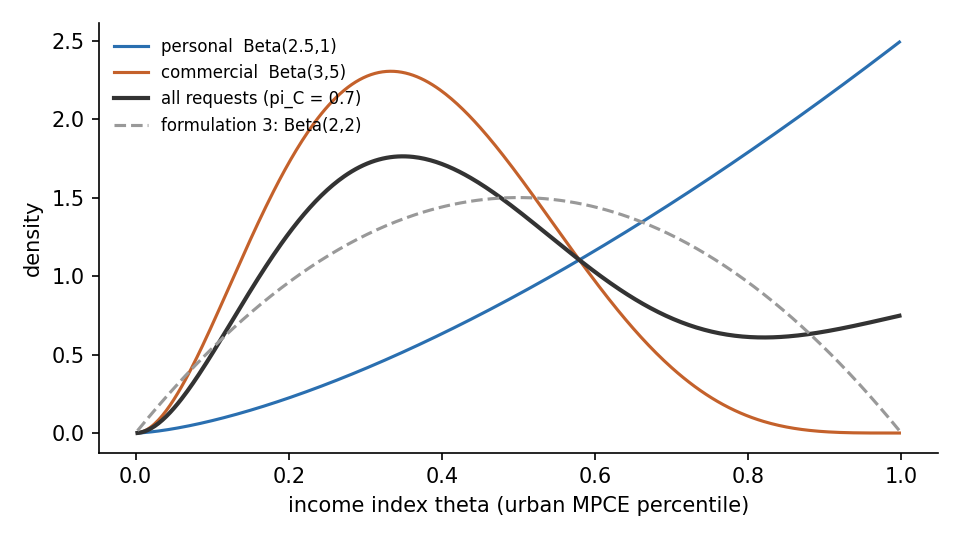
\includegraphics[width=0.78\textwidth]{data/calibration_densities.png}\\
{\small Income densities: personal Beta(2.5,1), commercial Beta(3,5), all requests with $\pi_{\mathrm C}=0.7$, and formulation 3's Beta(2,2).}
\end{center}
The population is bimodal: rich personal owners (around 0.7--1) and lower-middle-income commercial drivers (around 0.2--0.5); the mean income index of all requests is 0.48, close to formulation 3's 0.5, but the shape is very different. In the dataset (\texttt{data/}) the same draws give 69\,\% commercial EVs over all files.

%=====================================================================
\section{Experiments}
\label{sec:exp}

Each experiment changes one input at a time and is solved with both methods on the 560 Solomon instances (56 files, $n=10,\dots,100$), exactly as the baselines. Order (user, 22 Nov 2026): first E5 and E6, then E1, E2 and E8. The baseline value is not solved again.

{\small
\begin{tabularx}{\textwidth}{@{}p{0.6cm}>{\raggedright\arraybackslash}p{3.4cm}>{\raggedright\arraybackslash}p{4.6cm}X@{}}
\toprule
\# & \textbf{Factor} & \textbf{Variants (baseline in brackets)} & \textbf{Question} \\
\midrule
E5 & Value of charging time at $\theta=1$ & personal $c^{\mathrm C,\mathrm P,1}$ $\pm25\%$; commercial downtime rate $\omega^{1}$ (with $c^{\mathrm Q,\mathrm C,1}$) $\pm25\%$ & How sensitive is the van share of each segment to the most influential assumed value? \\[3pt]
E6 & Money sensitivity at $\theta=0$ & $\mu^{\mathrm P,0}$ $\pm25\%$; $\mu^{\mathrm C,0}$ $\pm25\%$ & The same for the coefficient with the largest elasticity on $Z$. \\[3pt]
E1 & Van tariff $p^{\mathrm M}$ & $p^{\mathrm M}=p^{\mathrm F}$ (no premium), (base), higher & Who gets vans, by segment and income, at what cost to the operator and to equity? \\[3pt]
E2 & Van fleet and seats & $|M|$ fewer / more; $Q_m$ fewer / more (one at a time) & Where does another van or seat pay off, and where is capacity idle? \\[3pt]
E8 & Van battery $B_m$ & larger & Is van recharging worth modelling? If $Z$ barely moves ($<1\%$), drop it. \\
\bottomrule
\end{tabularx}}

The values are in \texttt{common/experiments.json}. \textbf{MILP}: each variant runs the complete model with the baseline settings (time limit, workers, threads, warm start). \textbf{RL}: each variant gives two runs, the baseline policy applied to the changed inputs (zero-shot: its features read the coefficients, costs and fleet of each instance) and a policy retrained on the variant with the baseline recipe. \textbf{Measures}, on instances valid in both the variant and the baseline: change of $Z$, of the operator's and of the customers' cost; van share of free-choice EVs per segment and per income band; vans and seats used; queues, downtime and money paid per segment; for RL also the gap to the MILP of the same variant.

\textbf{What theory predicts} (Section~\ref{sec:theory}). E5 personal moves mostly the personal van share (driver-free benefit), E5 commercial the commercial van share in congested instances (downtime saved). E6 shifts low-income customers of the changed segment between FCS and van through $\mu^{s}\Pi_i$; its effect on $Z$ is direct (every tariff and drive term). E1 at $p^{\mathrm M}=p^{\mathrm F}$ removes the premium from $\Pi_i$ (only the saved drive cost $-c^{\mathrm{EV}}d_{if}$ remains), so the money channel favours the van and the choice is driven by $\kappa_i$, the saved downtime (commercial) and the driver-free benefit (personal). E2: more vans help most where seats bind; more seats where vans are idle at the depot. E8: the battery limit binds rarely in formulation 3, so $Z$ should move little.

%=====================================================================
\section{Implementation}
All code is in \texttt{2026-11-22\_formulation\_4/}: \texttt{data/} (complete dataset: the 56 Solomon and 60 Gehring--Homberger files with segment and $\theta$ per EV, calibration), \texttt{common/} (parameters, data reader, plan checker, result schema, analysis, experiment runner), \texttt{baseline\_MILP/} (Gurobi model of this document), \texttt{baseline\_RL/} (attention policy trained with REINFORCE, segment-aware inputs), and one folder per experiment and method (\texttt{E5\_value\_of\_charging\_time\_MILP}, \dots\_RL, \dots). Every plan, from either method, is scored by the same independent checker of constraints (2)--(23) and objective \eqref{eq:obj}.

%=====================================================================
\section{Changes with respect to formulation 3}
\begin{enumerate}[itemsep=2pt]
  \item \textbf{Use segment} $s_i\in\{\mathrm P,\mathrm C\}$ per EV, drawn as Bernoulli$(\pi_{\mathrm C})$; the income index is drawn per segment, $\theta_i\mid s_i\sim F_{s_i}$.
  \item \textbf{Sensitivities per segment}: $\mu^{s}(\theta)$, $c^{a,s}(\theta)$, $W^{s}(\theta)$, each with its own end points.
  \item \textbf{Commercial time = downtime}: $c^{\mathrm D,\mathrm C}=c^{\mathrm C,\mathrm C}=c^{\mathrm V,\mathrm C}=\omega(\theta)$, $c^{\mathrm Q,\mathrm C}\ge\omega$; no driver-free benefit from a van.
  \item \textbf{Calibrated distributions} (Section~\ref{sec:calib}) replace formulation 3's Beta$(2,2)$: $\pi_{\mathrm C}=0.7$, Beta$(2.5,1)$ for personal, Beta$(3,5)$ for commercial.
  \item Objective, variables and constraints (1)--(23) keep their form; the model size is unchanged.
\end{enumerate}

\end{document}
